\documentclass[twoside]{article}
\usepackage{microtype, fontspec}
\usepackage{textcomp, gensymb, amsmath, mathtools, siunitx, unicode-math}
% Page layout
\usepackage[a4paper, margin=20mm, headheight=12.0pt]{geometry}
\usepackage{fancyhdr, multicol, graphicx, caption, tabu, longtable, float, booktabs, tabularx, listings, xcolor, pdfpages, subcaption, titling, titlesec, enumitem, url, currency, pdflscape, ltxtable}
\usepackage[toc,page]{appendix}
\usepackage[style=ieee, backend=biber]{biblatex}
\usepackage[thinc]{esdiff}
\usepackage[colorlinks=true, linkcolor=blue, citecolor=red]{hyperref}

% Typefaces
\setmonofont{Iosevka SS15}
% \setmainfont{IBM Plex Sans}
\setmainfont{Latin Modern Sans}
% \setmonofont{Cascadia Code}
\setmathfont{Latin Modern Math}

% Listing Format
\lstset{language=C++,
        basicstyle=\small\ttfamily,
        numberstyle=\ttfamily,
        numbers=left,
        breaklines=true,
        tabsize=4,
        keywordstyle=\color{listingblue},
        commentstyle=\color{grey},
        captionpos=b}

% Maths formatting
\newcommand\ddfrac[2]{\frac{\displaystyle #1}{\displaystyle #2}}

% Colors
\definecolor{listingblue}{HTML}{2196f3}
\definecolor{blue}{HTML}{0069c0}
\definecolor{grey}{HTML}{9e9e9e}

% siunitx unit shortening
\newcommand{\amp}{\ampere}
\newcommand{\m}{\metre}
\DeclareSIUnit\vpp{\text{\ensuremath{V_{\textup{p-p}}}}}
\DeclareSIUnit\voltdc{\text{\ensuremath{VDC}}}

% Currency
\DefineCurrency{USD}{name={dollar}, plural={dollars}, symbol={\$}, iso={USD}, kind=iso, base=2, cents=true, pre=true}

% Figure
\newenvironment{Figure}
    {\par\medskip\noindent\minipage{\linewidth}}
    {\endminipage\par\medskip}

% Table formatting
\renewcommand{\arraystretch}{1.75}
\setlength{\tabcolsep}{5pt}
% \captionsetup[table]{skip=0pt}

% Bibliography
\addbibresource{TermThreeProject.bib}
\nocite{*}

% Header and footer
% Title page
\fancypagestyle{plain}{
    \fancyhf{}
    \fancyhead{}
    \fancyfoot[RO,LE]{\thepage}
    \renewcommand{\headrulewidth}{0pt}
}

% Normal pages
\pagestyle{fancy}
\fancyhf{}
\fancyhead{}
\fancyfoot[R]{\thepage}
\fancyfoot[L]{}
\renewcommand{\headrulewidth}{0pt}
\pagenumbering{roman}

% Start Document
\begin{document}

% Cover Sheet

% Title Page
\begin{titlingpage}
    {\centering
    \vspace*{3cm}
    {\LARGE\textbf{Arduino Shield HeadLight}\\}
    \vspace{1cm}
    {\textbf{Edward Manson (75953196)}\\}
    {\textbf{Alex Stiles (18120890)}\\}
    \vspace{1cm}
    {\today}
    \vfill
    \noindent
    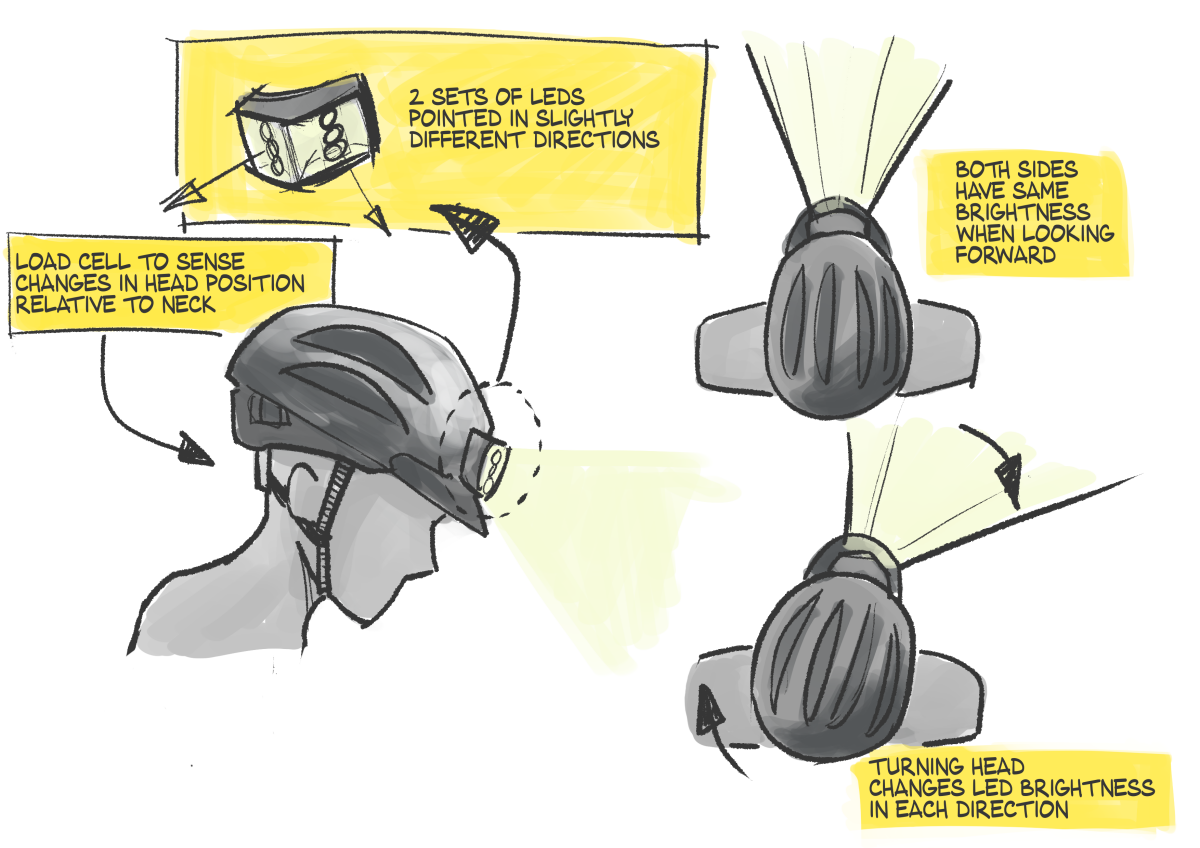
\includegraphics[width=0.75\linewidth]{headlamp-project-concept.png}
    \vfill}
\end{titlingpage}

% ToC

{\hypersetup{linkcolor=black}
\tableofcontents
\listoffigures
\listoftables
\lstlistoflistings}
\newpage

% Update Footer
\pagenumbering{arabic}
\fancyhead[C]{ENEL200}
\fancyhead[RE,LO]{Arduino Shield HeadLight}
\fancyfoot[C]{Edward Manson \& Alex Stiles}

\section{Introduction}

\section{Background}
    \noindent
    \begin{figure}[H]
        \centering
        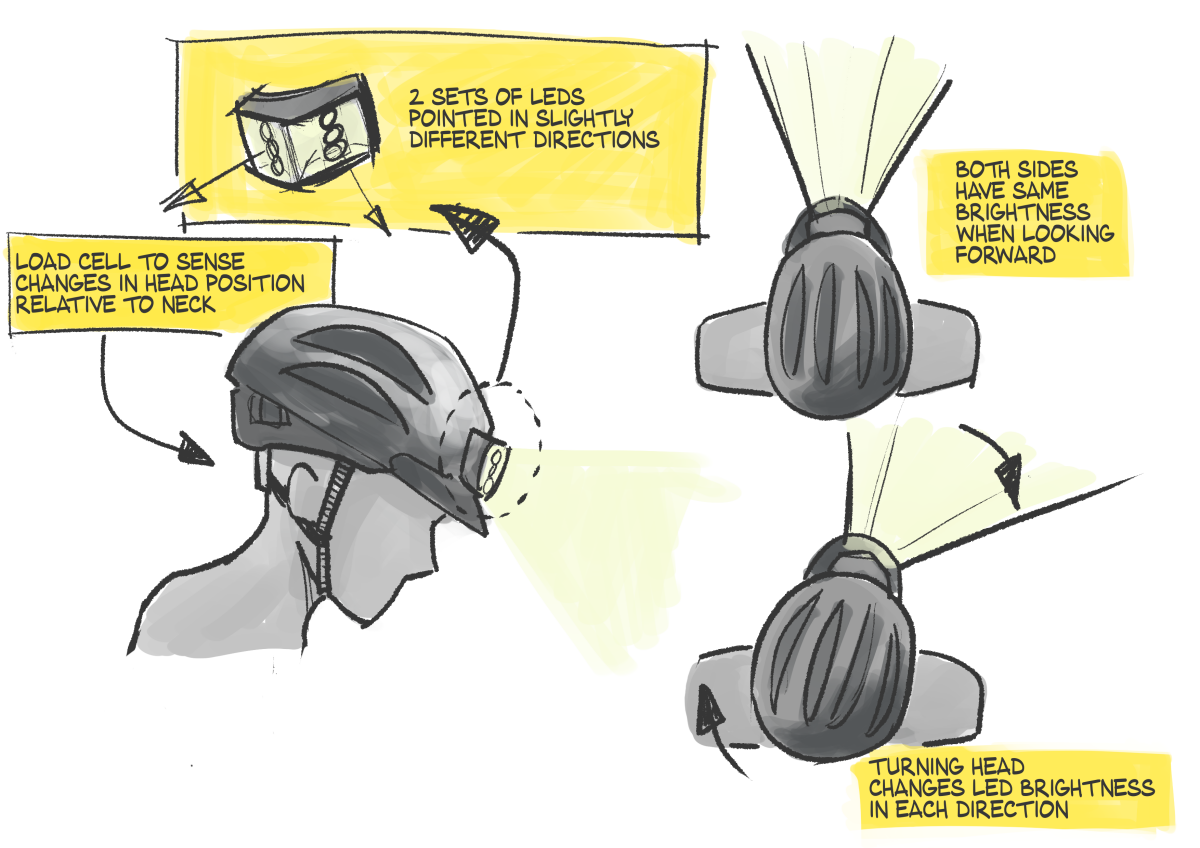
\includegraphics[width=0.75\textwidth]{headlamp-project-concept.png}
        \caption{A sketch of the HeadLight}
        \label{fig:sketch}
    \end{figure}

\section{Requirements \& Specifications}
    \subsection{Requirements}
    \subsection{Specifications}

\section{Design Overview \& Rationale}
    \noindent
    \begin{figure}[H]
        \centering
        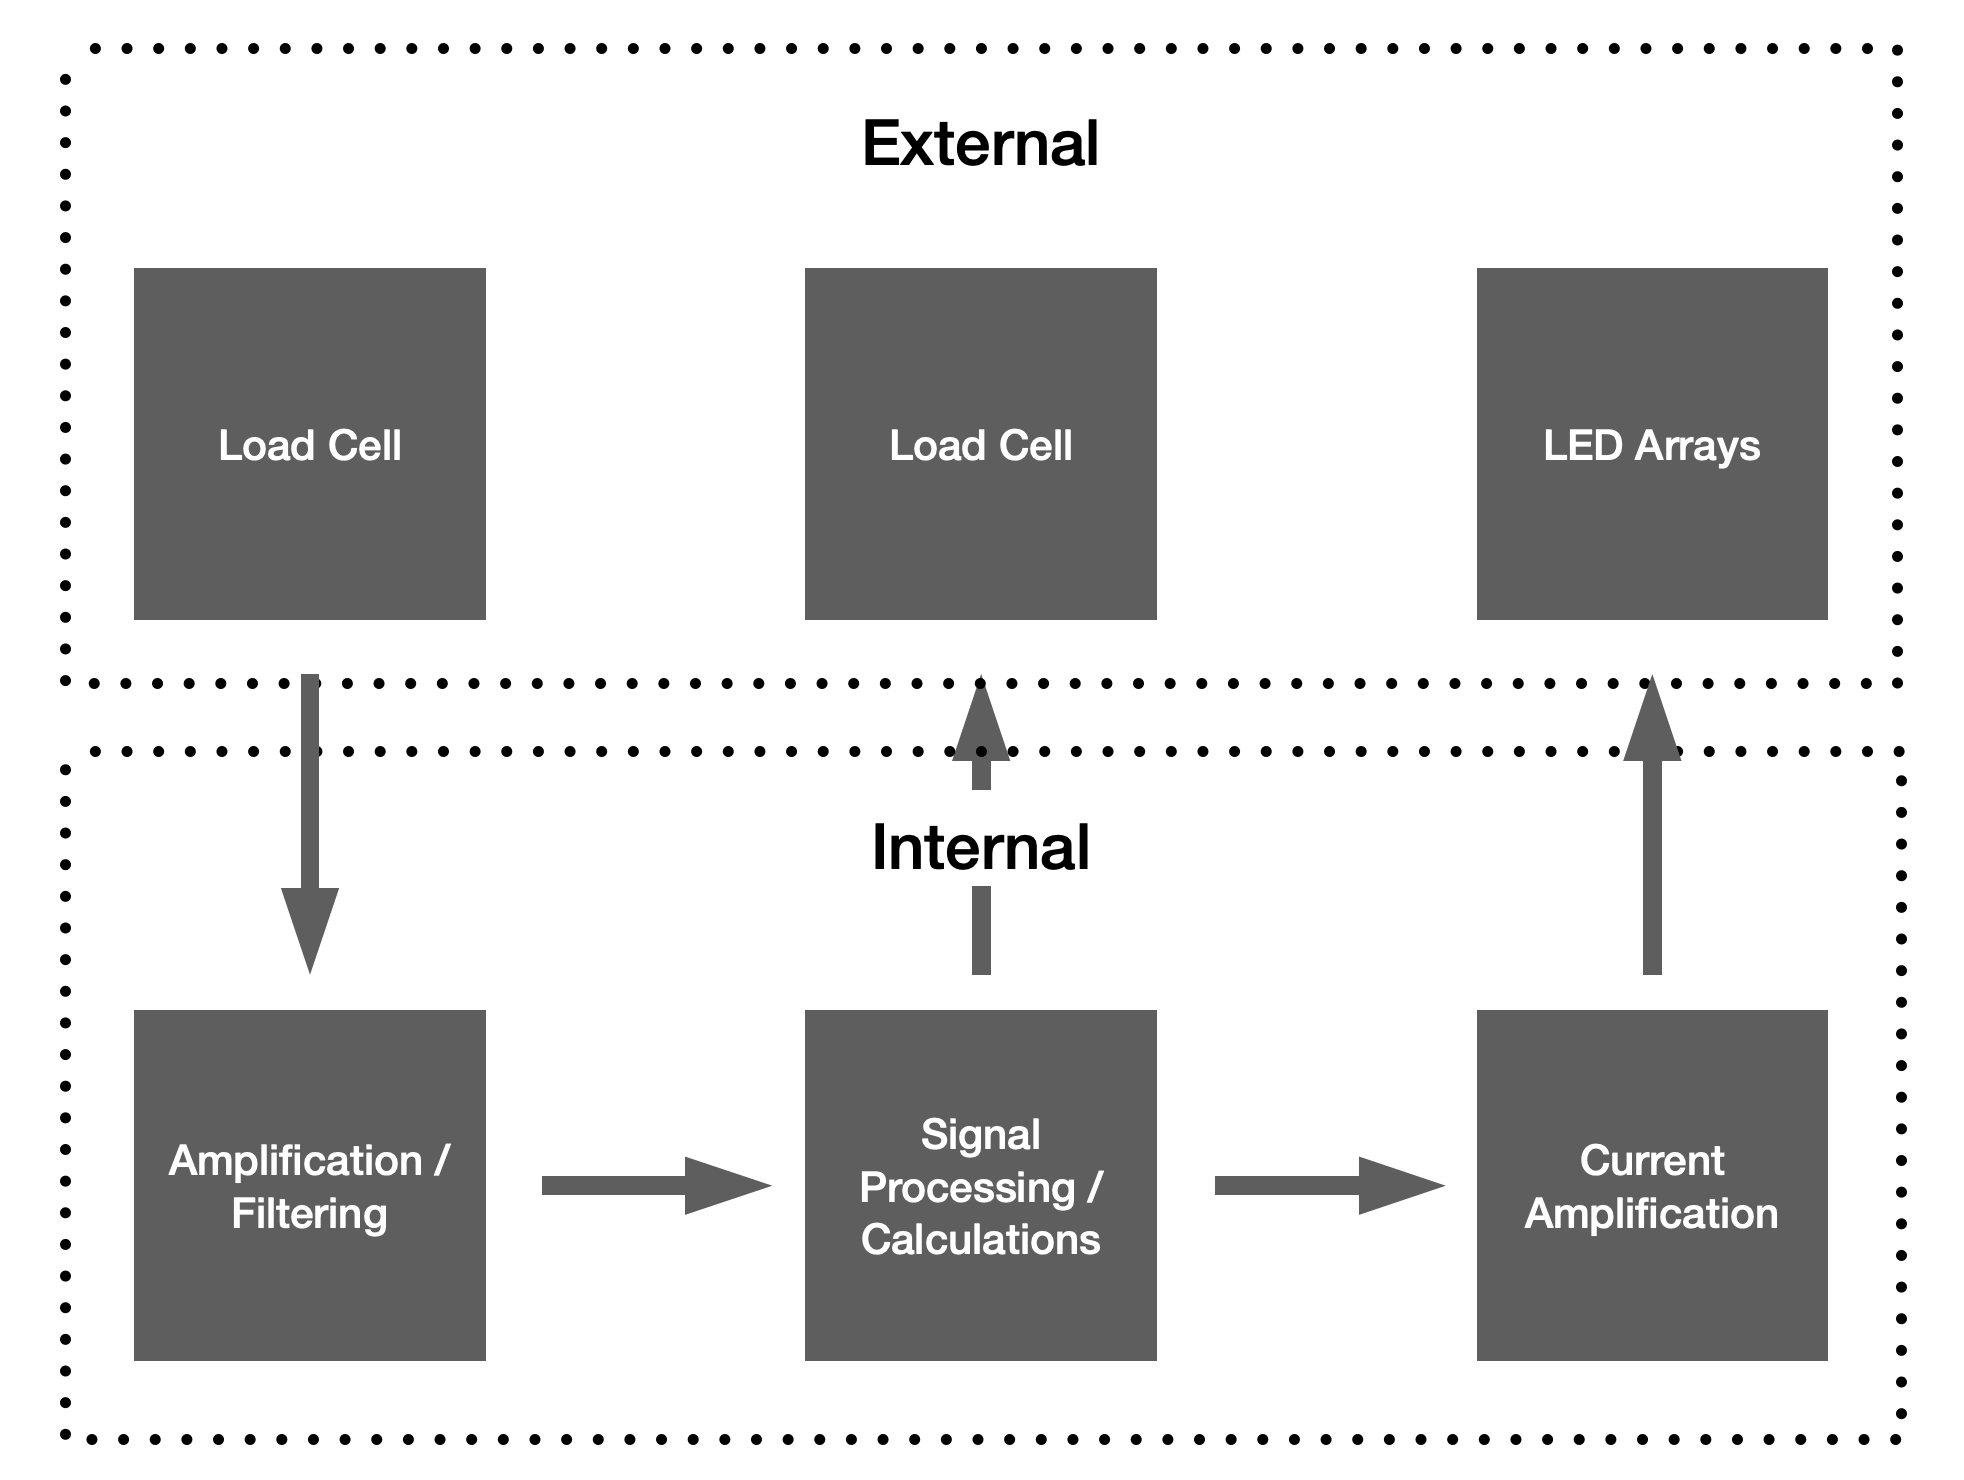
\includegraphics[width=0.75\textwidth]{block_diagram.png}
        \caption{A block diagram of the function of the HeadLight}
        \label{fig:block}
    \end{figure}

    \subsection{Arduino Shield}
        \paragraph{}
        A load cell is used to measure the force of the head rotation, which has an internal Wheatstone bridge. The output from the Wheatstone bridge goes into an instrumentation amplifier. The instrumentation amplifier consists of non-inverting amplifiers on the output of the Wheatstone bridge, which then goes into a differential amplifier, as shown in figure \ref{fig:inamp}. The output of the differential amplifier goes into an LC low pass filter to remove high-frequency noise.
        \noindent
        \begin{figure}[H]
            \centering
            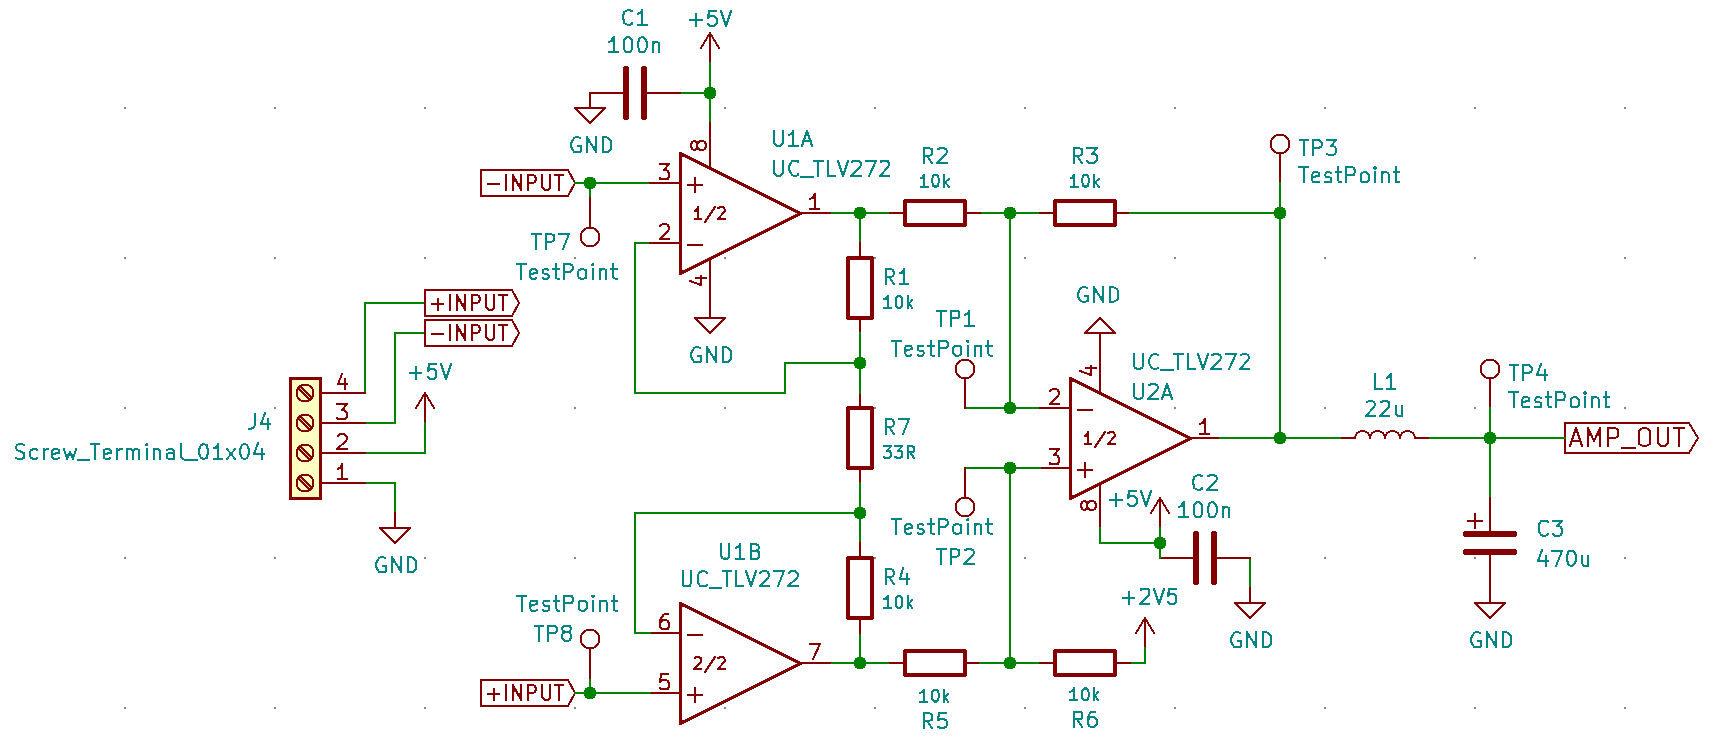
\includegraphics[width=\textwidth]{inamp.png}
            \caption{The layout of the instrumentation amplifier.}
            \label{fig:inamp}
        \end{figure}
        The output of the differential amplifier can end up being a negative value, as the Arduino can not read negative voltage, and there is no negative supply for the differential amplifier; the differential amplifier has to be biased. A voltage reference was constructed out of a voltage divider of equal values and a buffer to bias the instrumentation amplifier (shown in figure \ref{fig:vref}).
        \noindent
        \begin{figure}[H]
            \centering
            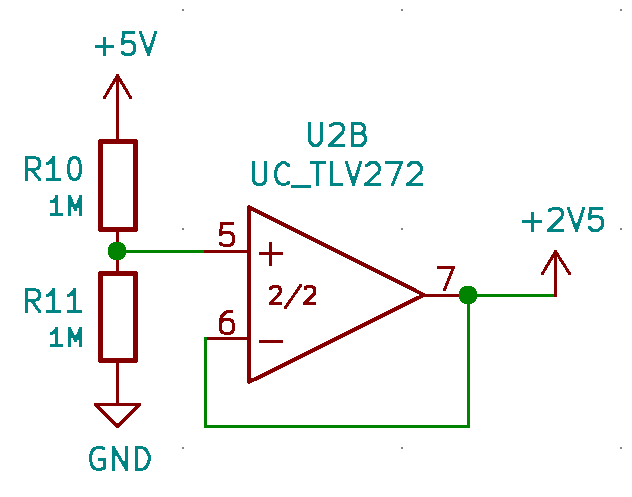
\includegraphics[width=0.75\textwidth]{vref.png}
            \caption{The layout of the voltage reference.}
            \label{fig:vref}
        \end{figure}
        For each LED array, the PWM output from the Arduino goes into the gate of a MOSFET. The current limiting resistor is connected to the anode of the LEDs, and the cathode of the LEDs is connected to the drain of the MOSFET.
        \noindent
        \begin{figure}[H]
            \centering
            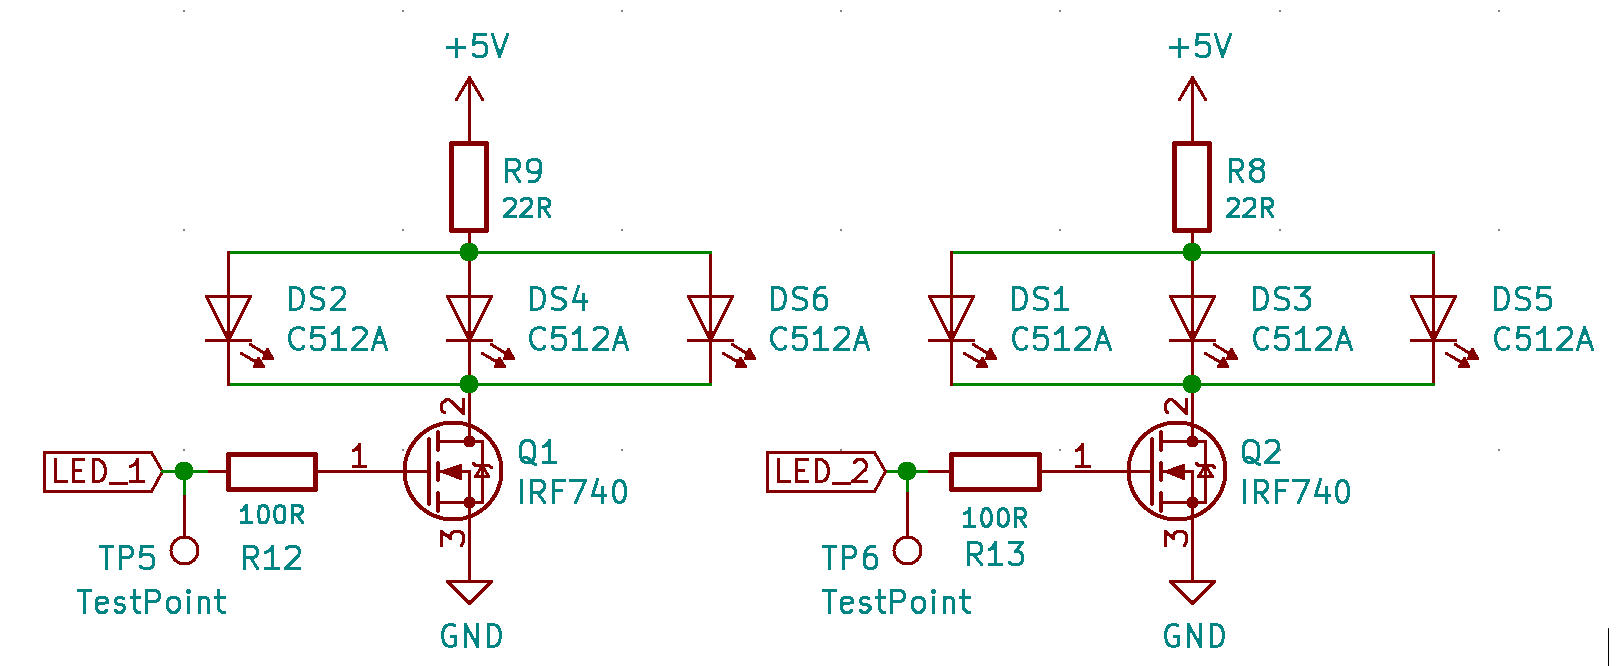
\includegraphics[width=0.75\textwidth]{ledarray.png}
            \caption{The layout of the LED arrays.}
            \label{fig:led}
        \end{figure}

        \subsubsection{PCB Layout}
        \paragraph{}
        The PCB was laid out to ensure that the ground plane would have no cuts, maximising EMC performance. Decoupling capacitors were placed right next to the power pins of the ICs. Additional care was taken so that traces were not too close to any antipads, as having traces too close to antipads can worsen EMC \cite{emc}. Test points were added so that we can troubleshoot any problems when assembling the prototype. 1x1 header were used as ground test points so that the ground clip of the oscilloscope probe can be attached.

        \subsubsection{Amplifier}
        \paragraph{}
        An instrumentation amplifier was chosen to amplify the signal from the load cell. The instrumentation amplifier consists of two non-inverting amplifiers, of which the outputs go into a differential amplifier. As the Arduino cannot read negative voltages, nor is there a negative supply, the differential amplifier was biased with \SI{2.5}{\volt}. This results in the positive difference being between \SI{2.5}{\volt} and \SI{5}{\volt}, and the negative difference is between \SI{0}{\volt} and \SI{2.5}{\volt}. A one op-amp differential amplifier has an extremely low input impedance; thus the Wheatstone bridge must have a matched impedance. A two op-amp instrumentation amplifier would require one less package but would be less stable than the three op-amp instrumentation amplifier. The three op-amp instrumentation amplifier also has a spare op-amp which is then utilised for the voltage reference.

        An initial gain of \SI{24}{\ohm} was calculated (as shown in equation \eqref{eq:g4}) \cite{ti:sloa034}, but after some test on a breadboard, the gain was changed \SI{33}{\ohm}. This was partly due to the load cell to measure \SI{\sim 50}{\percent} more than rated \cite{htc:tal221}.
        \begin{align}
            V_{O} &= \left[ \left(\text{Sig}^{+}\right) - \left(\text{Sig}^{-}\right)\right]\left[\frac{R_{4}}{R_{2}} \left[\frac{2R_{f}}{R_{g}} + 1\right] \right] \label{eq:g1}\\
            R_{g} &= \ddfrac{2R_{f}}{\left[\frac{V_{O}}{\left(\text{Sig}^{+}\right) - \left(\text{Sig}^{-}\right)} \frac{R_{2}}{R_{4}} \right]-1} \label{eq:g2}\\
            &= \ddfrac{2 \cdot \SI{10}{\kilo\ohm}}{\left[\frac{\SI{2.5}{\volt}}{\SI{3}{\milli\volt}} \frac{\SI{10}{\kilo\ohm}}{\SI{10}{\kilo\ohm}} \right]-1} \label{eq:g3}\\
            &= \SI{24.03}{\ohm} \label{eq:g4}
        \end{align}

        \subsubsection{Voltage reference}
        \paragraph{}
        A voltage divider was used to produce \SI{2.5}{\volt} to bias the differential amplifier. It was decided to use a buffer on the output of the voltage divider so that the common-mode rejection error is minimised. This is due to the op-amp's low output impedance, which does not introduce any noticeable common-mode rejection error. A \SI{2.5}{\volt} Zener diode would have been preferred. The resistors in the voltage divider have tolerances and therefore may not give exactly \SI{2.5}{\volt}; however, \SI{2.5}{\volt} Zener diodes were not available from the store. \SI{1}{\mega\ohm} resistors were chosen to limit the current and thus power consumption.

        \subsubsection{Filter}
        \paragraph{}
        A filter was used to filter out high-frequency noise from the load cell. The filter was chosen to be an LC filter. An RC filter could have been used, but it would have caused the signal's voltage to drop slightly due to the voltage drop across the resistor. The LC filter does require more space on the PCB, but the PCB had enough room for the capacitor and the inductor. LC filters also have better attenuation as the attenuation slope is twice as steep as an RC filter. The filter was placed on the output of the differential amplifier. If filters were placed on the inputs of the differential op-amp, more components would be needed, and there would not be enough space on the board. A \SI{22}{\micro\henry} inductor was chosen due to its availability in the electronics store. A \SI{470}{\micro\farad} capacitor was selected as a compromise of its physical size, cutoff frequency, and availability. The cutoff frequency was found to be \SI{1.595}{\kilo\hertz}, as shown below:
        \begin{align}
            f &= \ddfrac{1}{2 \pi \sqrt{L C}} \label{eq:f1}\\
            &= \ddfrac{1}{2 \pi \sqrt{\SI{22}{\micro\henry} \SI{470}{\micro\farad}}} \label{eq:f2}\\
            &= \SI{1.595}{\kilo\hertz} \label{eq:f3}
        \end{align}

        \subsubsection{LED arrays}
        \paragraph{}
        Each LED array has a MOSFET; this was done to have enough current supplied to the LEDs. The pins that can output PWM are only able to supply \SI{40}{\milli\amp}, so the outputs from these pins were connected to the gates of the MOSFETs. This allows the LEDs to take full current and are thus brighter. IRF740 MOSFETs were chosen due to their availability in the store and their low resistance. They have a max current of 10 A, so more LEDs can be added if required. The low resistance of the IRF740 (\SI{0.55}{\ohm}), reduces the power losses when the MOSFET is on. Individual resistors could have been matched to each LED; however, this would increase the number of components and take up extra space on the PCB. \SI{100}{\ohm} resistors were placed between the PWM output from the Arduino and the gate of the MOSFETs, this was done to minimise ringing and to limit current.

    \subsection{Microcontroller Overview}
        \paragraph{}
        The microcontroller selected for the HeadLight prototype was the Arduino Uno Rev 3. The Arduino Uno provides many advantages over other options. Mainly, it provides a simple interface, through C++ libraries, for accessing core hardware facilities and corresponding functionality, such as GPIO and PWM manipulation. The HeadLight design makes extensive use of both GPIO pins and PWM output, therefore having the ability to access and manipulate these rapidly is important to expedite the early prototyping stages. 

        We wrote the software for the Arduino in C as opposed to C++. C++ is the natural choice as the Arduino libraries are written in C++, and the source code is compiled as C++. Still, after analysing the advantages and disadvantages of each option, we decided that C was the better choice. The benefits of using C over C++ are as follows:
        \begin{itemize}
            \item We collectively have more experience with C than C++, making collaboration easier and coding quicker.
            \item The Arduino doesn't provide the C++ standard library (ref), as it uses too much dynamic memory.
            \item Software written in C is likely to be easier to port to another, more appropriate microcontroller if the product matures past the prototyping stage. 
        \end{itemize}
        There are disadvantages to this decision, which we took into due consideration:
        \begin{itemize}
            \item In the way we would've written the code, C++ is easier to read to those without C/C++ experience. The primary advantage of C++ in this context is the use of the OOP paradigm through classes, encapsulation, and polymorphism. This programming style would be more similar to those with Python experience than the procedural style of C. 
            \item There is some essential boilerplate required in the header files containing function prototypes. This boilerplate is a set of preprocessor directives that ensure the C++ linker doesn't mangle the function names. 
            \item Following the previous point, C++ is a superset of C, meaning all C code is valid (if not best practice) C++ code. Unfortunately, this is not true in the other way. Therefore, to use C++ code in C, a linker library must be written, which requires significant work. Thus, the Arduino libraries that provide access to the GPIO pins and PWM functionality cannot be accessed in functions linked as C code. Consequently, we can only use the Arduino library functions within the \texttt{main.ino} file. 
        \end{itemize}

        \subsubsection{Software Functionality}
            In the whole system seen figure \ref{fig:block}, the Arduino's job is to calculate and process the signal from the load cell after it has been amplified and filtered and utilise that information to determine the required PWM outputs of the two LED arrays.  
            The software has two modes programmed:
            \begin{itemize}
                \item The first is the `follow' mode, which changes the intensity of the LED array associated with the direction of head rotation, as seen in Figure \ref{fig:sketch}. For example, if someone was looking \SI{90}{\degree} left, the left LED array would be full intensity while the right LED array would be off. This is the mode the headlight is in when turned on.
                \item The second is `full' mode, in which both of the LED groups are at full brightness regardless of the load cell state. 
            \end{itemize}
            \paragraph{Overview}
            When someone turns on the Arduino, it goes through an initial setup process. Once the Arduino has completed this, it enters a loop that handles all the sensor polling, calculations, and PWM output manipulation.
            A high-level overview of the loop that the Arduino runs through is as follows:
            \begin{itemize}
                \item Get the current button reading and debounce it: 
                \item \begin{itemize}
                        \item Update the mode if it is determined the user pressed the button
                    \end{itemize}
                \item Check if that either are true:
                \item \begin{itemize}
                        \item Poll the load cell and check if it has detected a deviation of at least \SI{0.1}{\volt}. 
                        \item Check if the mode has changed this loop. 
                        \item If either of these is true:
                        \item \begin{itemize}
                            \item Calculate and update the PWM outputs of the two LED arrays.
                        \end{itemize}
                    \end{itemize}
                \item Stop execution for \SI{20}{\milli\second} to reduce power usage while maintaining a high polling rate to detect button presses and rapid head movements.
            \end{itemize}
            A complete code listing can be found in Appendix \ref{appendix:listing}.
            \paragraph{Reading Load Cell Signal}
            Every time the Arduino loops, it polls the load cell to check if the currently read voltage differs from the previously read voltage reading by a defined constant, \texttt{DEVIATION\_VOLTAGE}, set to 0.1. The deviation check code snippet is shown below:
            \begin{lstlisting}
Deviation = (load_cell->voltage - read_voltage) > load_cell->deviation_voltage_breakpoint 
            \end{lstlisting}
            If this is true, the Arduino updates the load cell reading and other associated values, specifically strain and angle. The deviation flag is also set to true, which indicates that the PWM outputs of the LED arrays need to be updated.
            \paragraph{Calculating PWM Output}
            Once the Arduino has detected a sufficient deviation in load cell voltage, it can calculate the new PWM outputs. Assuming the mode is `follow', the amplified load cell voltage is mapped to the range of PWM output values \(\left[0, 255\right]\). The paraphrased code snippet used to get the left LED array PWM output is shown below. Constants have been substituted with their values for convenience. 
            \begin{lstlisting}
left_group_brightness = (uint8_t) round(((load_cell->voltage - COMMON_MODE_VOLTAGE) / load_cell->max_voltage) + 0.5) * 255);
            \end{lstlisting}
            This value is then rounded to the closest integer and cast to a \texttt{uint8\_t}, an unsigned 8-byte integer that can hold values \(\left[0, 255\right]\). The value for the right LED array is the max PWM write value minus the calculated value for the left LED array shown below:
            \begin{lstlisting}
right_group_brightness = (255 - group_one_brightness); 
            \end{lstlisting}
            \paragraph{Button}
            The Arduino switches between the modes by using a user interaction through a button. To ensure the button isn't triggered arbitrarily, we utilised two methods to reduce noise triggering. 

            Firstly, we used the Arduino's internal pullup resistor on the button, ensuring a logical high when the button is not pressed instead of a floating voltage. Unfortunately, this doesn't solve the problem of the button rapidly changing state when pressed and released. Therefore, secondly, the Arduino, through software, also debounces the button before its state is confirmed. The button must hold a different state (released after being pressed, for example) for \SI{20}{\milli\second} before being registered. \SI{20}{\milli\second} was determined to be a good intermediary between not interfering with user interaction and removing the rapid switching through testing. The function used to debounce the button state is shown below:
            \begin{lstlisting}
void debounce_state(Button_t* button, bool read_button_state, long unsigned current_time) {     

if (read_button_state != button->last_state) { 
    button->last_trigger_time = current_time; 
} 

if ((current_time - button->last_trigger_time) > button->debounce_delay) { 
    if (read_button_state != button->state) { 
        button->state = read_button_state; 
        if (button->state) { 
            button_clicked(button); 
        } 
    }
} 

button->last_state = read_button_state; 
            \end{lstlisting}

\section{Testing}
    The PCB will be assembled and attached to an Arduino. The code will be uploaded to the Arduino. The load cell will be manipulated, and the PWM signal will be probed using an oscilloscope. The duty cycle of the PWM signal will be compared to the expected duty cycle.
    The LEDs will then be connected, and the load cell manipulated to check that the LEDs behave as expected in terms of brightness and direction changes. 
    The load cell signal will be probed to ensure that the gain resistor is the correct value. This will be done by placing an appropriately \SI{100}{\gram} mass on the load cell and measuring the voltage that is output by the instrumentation amplifier.

\section{Conclusion}
    \paragraph{}
    This report detailed the prototyping process undertaken to test the feasibility of the HeadLight concept. We achieved our goal of developing a medium-fidelity prototype which allowed us to demonstrate the functionality of HeadLight. The prototype developed contained six distinct parts, as shown in the block diagram \ref{fig:block}. All the parts work together to implement the required functionality as well as the additional mode functionality. The load cell output first goes through an amplification and conditioning stage, which involves an instrumental amplifier and filtering section and takes place on the shield. The modified signal then enters the Arduino through a GPIO pin. The Arduino then determines if sufficient deviation has been detected to alter the PWM outputs. These outputs enter the gates of MOSFETs, which 'amplifies' the current received by the LED arrays. This general loop is what could be expected from a final product. The startup's design team has indicated that they know that the Arduino Microcontroller is not suitable long term for this project but is very applicable during the prototyping process. 

    Developing this prototype provided many insights into the advantages and disadvantages of design decisions set by the specifications, specifically related to the load cell. Although we didn't house the prototype in a helmet enclosure, we have concerns about using a load cell to detect head movement. Although the load cell could be attached to the helmet in such a way as to produce a reliable reading for purely horizontal deviation, we are worried that vertical head deviation could have unintended consequences. Therefore, if we undertook future prototyping, we would recommend switching to a gyroscope and accelerometers to attain head movement. This would provide more accurate, precise readings and more relevantly isolate movement on a specific axis. 

    Overall, we also have concerns about the ability of HeadLight to offer any appealing additional functionality. Further testing within context would have to be undertaken by stakeholders to establish if the HeadLight in its current form provides any significant advantage over a standard headlight.
    
\newpage
% Bibliography
\printbibliography

\newpage
\begin{appendices}
    \section{Applications of the Design Toolkit}
        \begin{center}
            \begin{longtable}{ p{0.2\linewidth} p{0.2\linewidth} p{0.5\linewidth}}
                \caption{Applications of the Design Toolkit} \label{table:designtoolkit}\\

                % First page header
                \toprule
                \textbf{Tool Type} & \textbf{Tool Name} & \textbf{Where/How Used} \\
                \midrule
                \endfirsthead

                % Normal page headers
                \multicolumn{3}{c}
                {{ \tablename\ \thetable{} -- continued from previous page}} \\
                \midrule
                \textbf{Tool Type} & \textbf{Tool Name} & \textbf{Where/How Used} \\
                \midrule
                \endhead

                % Normal page footers
                \midrule
                \multicolumn{3}{r}{\itshape continues on next page}\\
                \midrule
                \endfoot

                % Last footer
                \bottomrule
                \endlastfoot

                Strategy & Divide \& Conquer & Divide and conquer was used to split up the hardware design into:
                \begin{itemize}
                    \item Instrumentation amplifier
                    \item LED arrays and driver
                    \item \SI{2.5}{\volt} reference
                    \item LC filter
                \end{itemize} 
                The project itself was also divided up so that one person did the software, and the other person did the hardware. \\
                Design Principle & PCB layout & The layout of the PCB was done with the aim of complying with the PCB design rules, e.g. Having components neatly lined up, minimising acute angles of tracks, increasing clearance between components and tracks, and having high current tracks where needed. \\
                Design Principle & Schematic layout & The schematic was done with the aim to follow the layout guidelines, for example, using labels, using power ports, separating major parts of the circuit, and ensuring that the labels are clear and easy to read. \\
                Design Principle / Strategy & Modularity & The code was written with the aim to be modular, e.g. multiple header files and task specific files. \\
                Design Principle & Testability & Test points were added around the circuit to aid in easy testing of the circuit's function. \\
                Strategy & Get another perspective & Both the PCB and the schematic were checked by people other than the designer, such as the other group member and people external to the group. \\
                Building Block & Amplifier & An instrumentation amplifier was constructed out of operational amplifiers to appropriately amplify the signal from the Wheatstone bridge in the load cell. \\
                Building Block & Filter & An LC filter was used to filter out noise from the load cell, and to not attenuate the signal. \\
                Building Block & Buffer & A buffer was used to create a low impedance voltage reference. Buffers were also used on the output of the 
                Wheatstone bridge to provide a high impedance for the Wheatstone bridge so that the signal was not excessively attenuated. \\
                Building Block & Current Limiting Resistor & Current limiting resistors were usd to limit the gate current for the MOSFETs and the current through the LEDs. \\
                Building Block & Arduino microcontroller & The Arduino is the main controller for the circuit, it controls the brightness and reads the load cell. \\
                Background & Arduino programming & The functionality of the LED arrays is controlled by the Arduino through PWM signals which are manipulated using programming \\
                Building Block & Pull up resistor & An internal pull up resistor is used for the button. A pull up was chosen so that the internal pull up resistor could be utilised, keeping the parts count down.\\
                Building Block & Analog input & An analog input was used to read the amplified signal from the Wheatstone bridge of the load cell. \\
                Building Block & Digital output & Digital outputs were used for the MOSFETs that control the LEDs, amd for the auxillary output. Digital outputs are capable of outputting PWM.
            \end{longtable}
        \end{center}
    \newpage

    \section{Code}
        \label{appendix:listing}
        \lstinputlisting[caption=Button code., label=Listing:1]{../main/button.c}
        \lstinputlisting[caption=Button header code., label=Listing:2]{../main/button.h}
        \lstinputlisting[caption=LED group code., label=Listing:3]{../main/LED_Group.c}
        \lstinputlisting[caption=LED group header code., label=Listing:4]{../main/LED_Group.h}
        \lstinputlisting[caption=.LED group collection code, label=Listing:5]{../main/LED_Group_Collection.c}
        \lstinputlisting[caption=LED group collection header code., label=Listing:6]{../main/LED_Group_Collection.h}
        \lstinputlisting[caption=Load cell code., label=Listing:7]{../main/Load_Cell.c}
        \lstinputlisting[caption=Load cell code., label=Listing:8]{../main/Load_Cell.h}
        \lstinputlisting[caption=Main code., label=Listing:9]{../main/main.c}
        \lstinputlisting[caption=Voltage ADC code., label=Listing:10]{../main/voltage.c}
        \lstinputlisting[caption=Voltage ADC header code., label=Listing:11, captionpos=b]{../main/voltage.h}
        \lstinputlisting[caption=Main Arduino code., label=Listing:main, captionpos=b]{../main/main.ino}
    \newpage
    \section{Schematic}
        \label{appendix:schematic}
        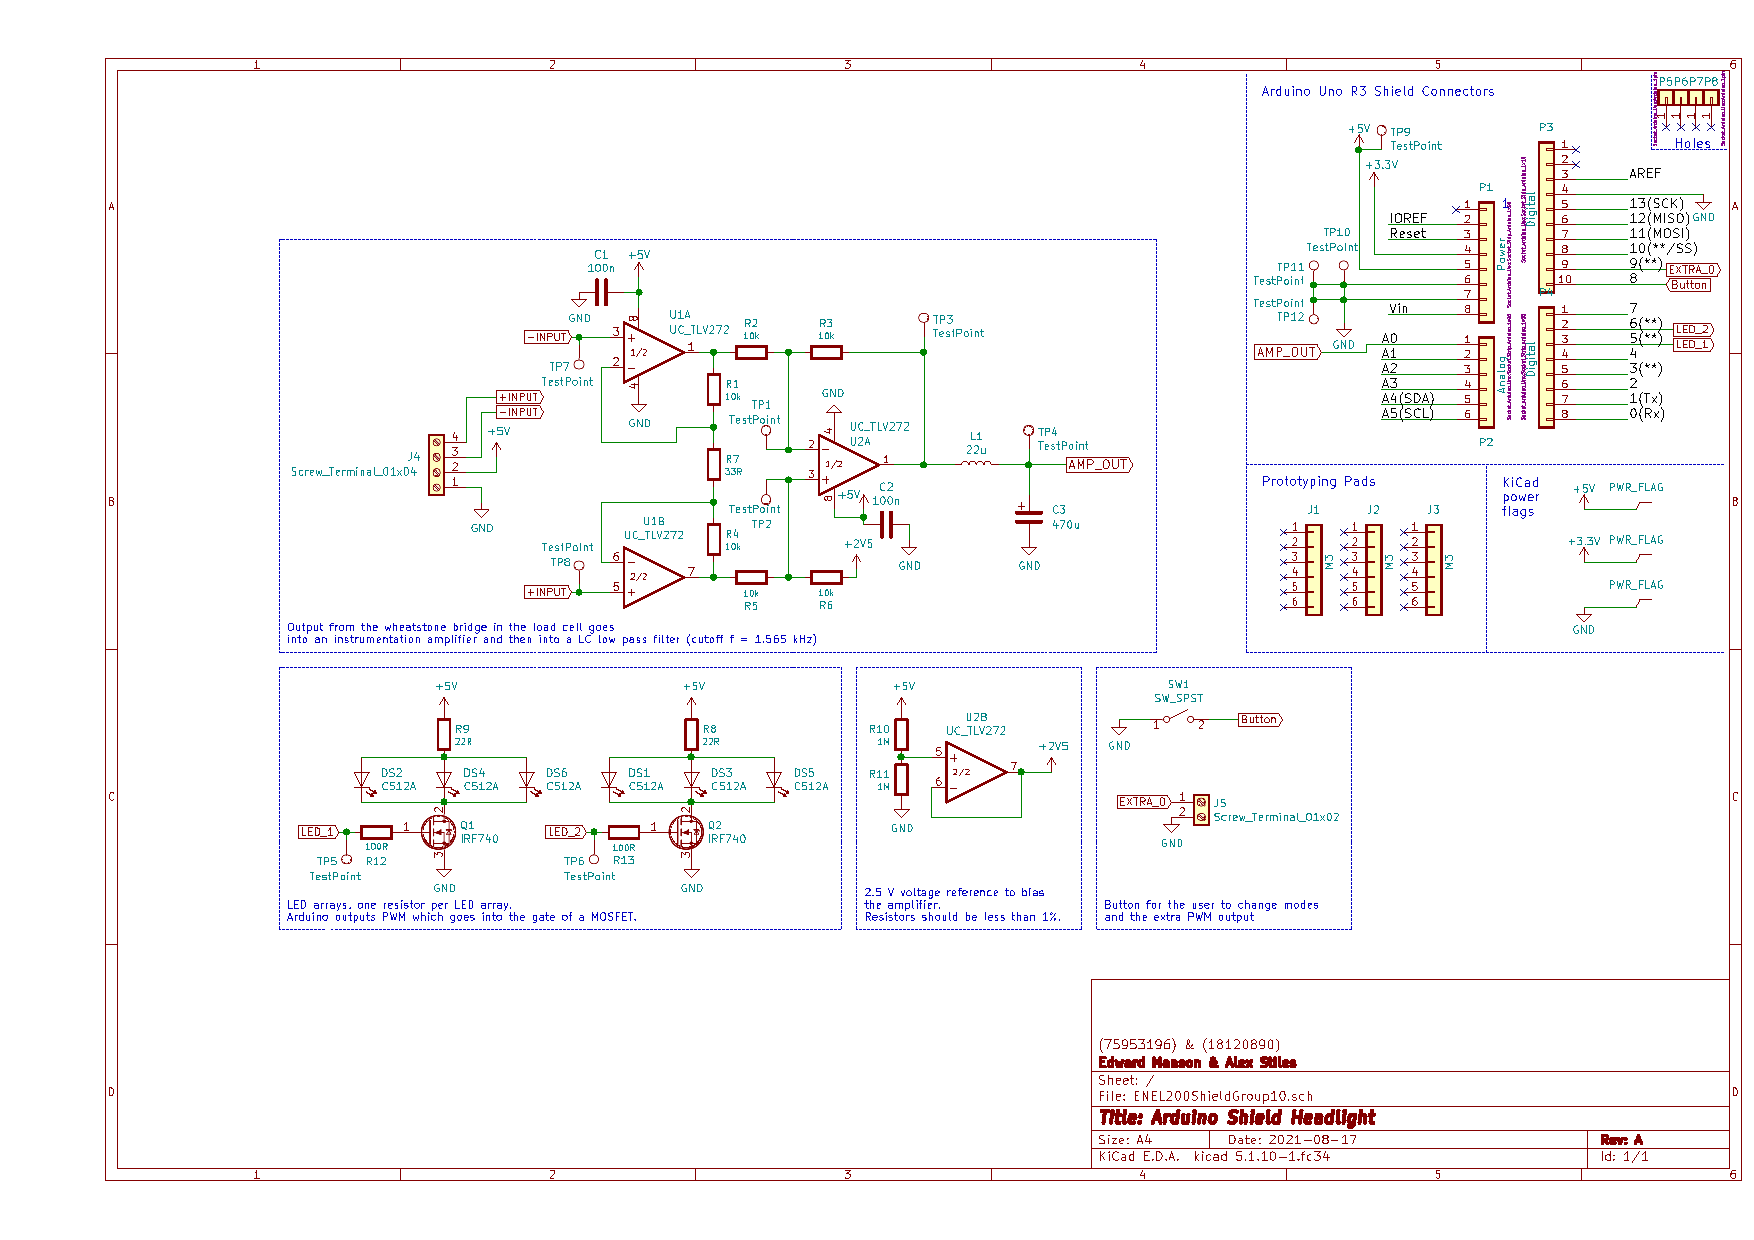
\includepdf[pages=-,landscape=true]{schematic.pdf}
    \newpage
    \section{Printed Circuit Board}
        \label{appendix:pcb}
        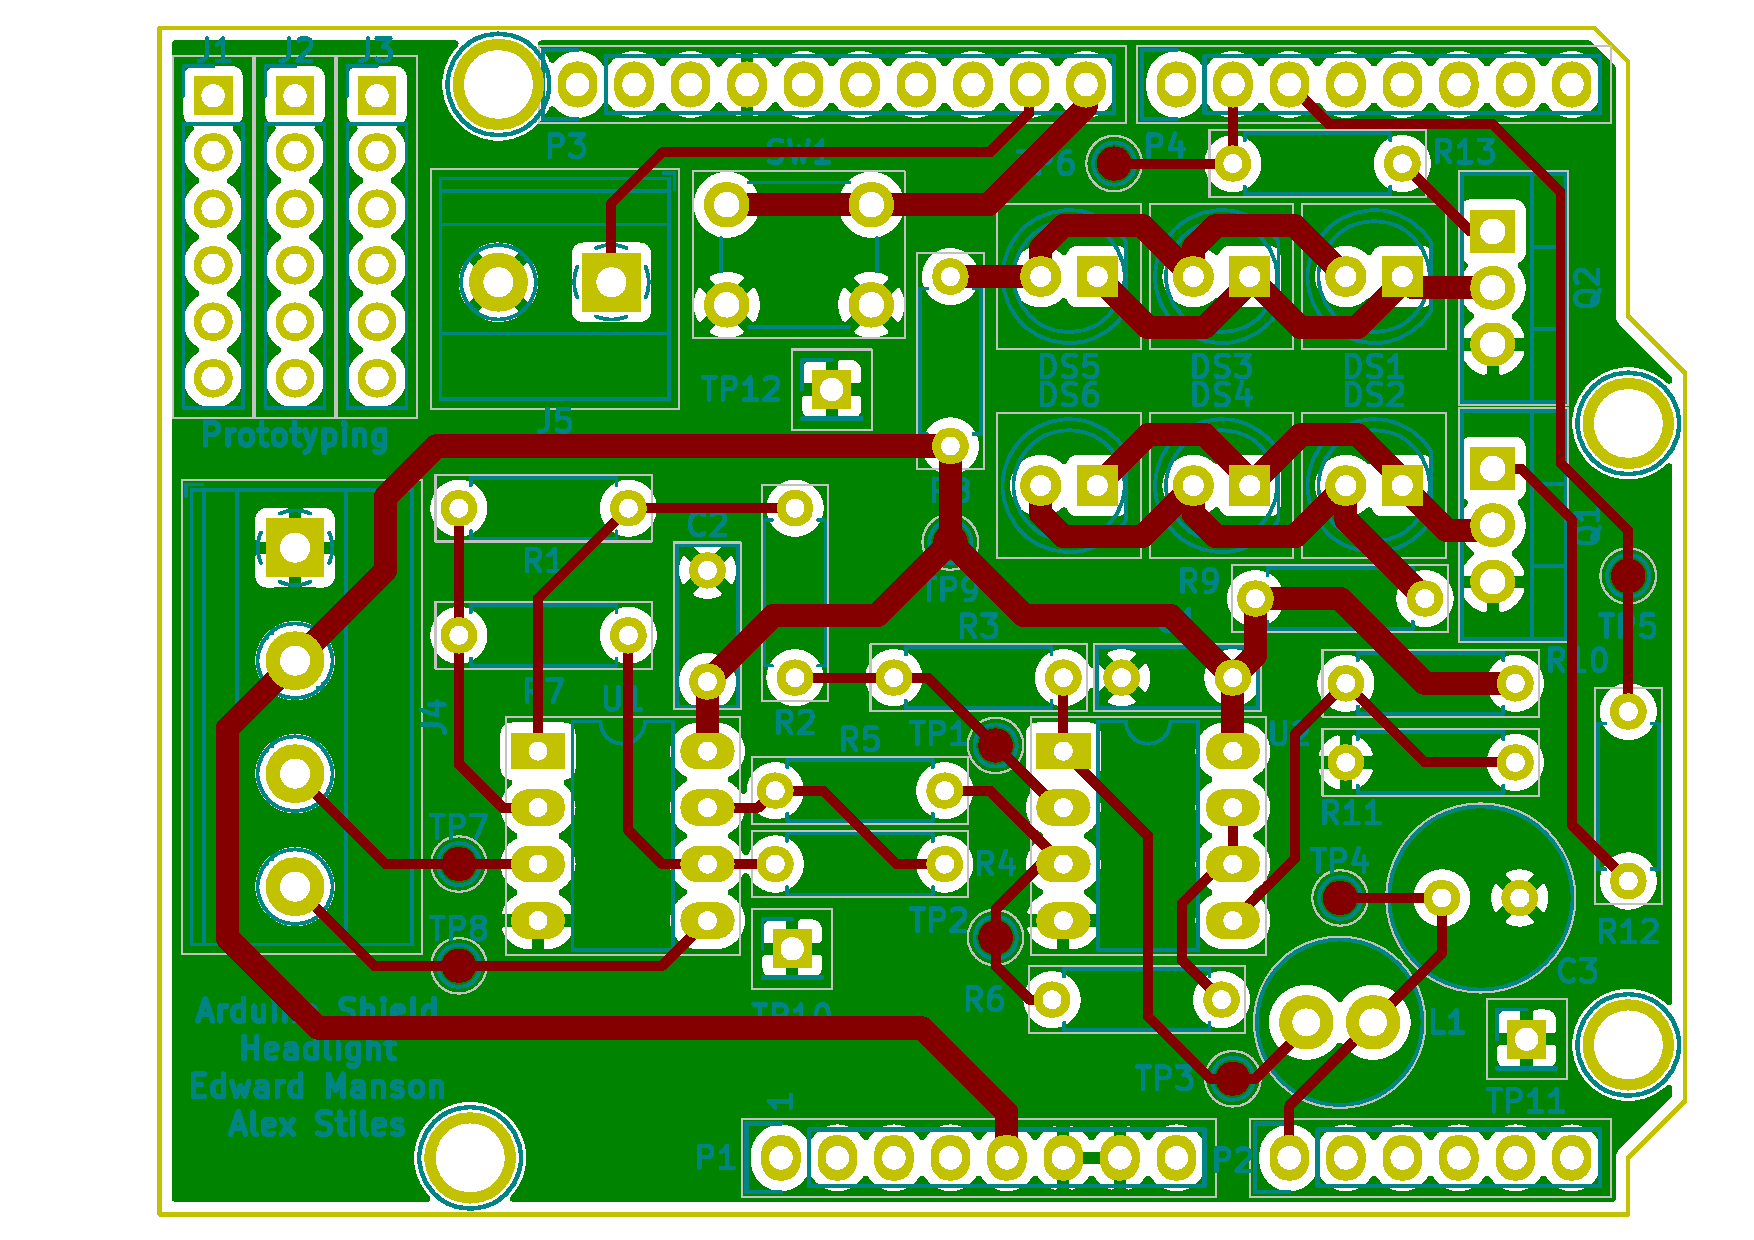
\includepdf[pages=-,landscape=true]{pcb.pdf}
    % \newpage
    % \section{Bill of Materials}
    %     \label{appendix:BOM}
    %     \noindent
    %     \begin{table}[H]
    %         \centering
    %         \begin{tabular}{ p{2.5cm} c l p{5cm} S }
    %             \toprule
                % Ref. & Qnty & Value & Description & {Price (individual per 100)} \\
                % & & & & {(\cUSD)}\\
                % \midrule
                % C1, C3, C4, C5, C7, C8 & 6 & \SI{100}{\nano\farad} & Tantalum capacitor & 0.21380 \\
                % C2, C6 & 2 & \SI{470}{\micro\farad} & Electrolytic capacitor & 0.14210 \\
                % D1 & 1 & 1N4007 & Diode & 0.06690 \\
                % IC1, IC2 & 2 & CD4026BE & Counter and seven segment display driver & 0.35620 \\
                % RV1, RV2 & 2 & \SI{1}{\mega\ohm} & Trim pot & 0.42300 \\
                % R3 & 1 & \SI{1}{\mega\ohm} & Resistor & 0.01480 \\
                % R4 & 1 & \SI{100}{\ohm} & Resistor & 0.01480 \\
                % R5 & 1 & \SI{4.7}{\kilo\ohm} & Resistor & 0.01480 \\
                % {R6, R7, R8, R9, R10, R11, R12, R13, R14, R15, R16, R17, R18, R19} & 14 & \SI{1.8}{\kilo\ohm} & Resistor & 0.01480 \\
                % R20 & 1 & \SI{150}{\kilo\ohm} & Resistor & 0.01480 \\
                % SW1 & 1 & SW\_SPDT & Switch, single pole double throw & 1.27990 \\
                % SW2 & 1 & SW\_Push\_SPDT & Momentary Switch, single pole double throw & 1.17890 \\
                % U2 & 1 & LM358 & Dual operational amplifier & 0.22730 \\
                % U3, U4 & 2 & SRC56-11SRWA & 7 segment hyper red LED, common cathode & 0.51800 \\
                % U5 & 1 & 78L05 & Positive \SI{100}{\milli\amp} \SI{30}{\volt} Linear Regulator, Fixed Output \SI{5}{\volt} & 0.13440 \\
                % U6 & 1 & CD4047B & Monostable/Astable Multivibrator & 0.41550 \\
                % \midrule
                % & 38 & & & 7.73070 \\
        %         \bottomrule
        %     \end{tabular}
        % \end{table}
\end{appendices}

\end{document}